%% Week 37 -- Cross-validation revisited, gradient descent, momentum and
%% automatic differentiation
%% Sources: Sections 2.12 and 3.14 of chapter3.tex (the cross-validation
%% recap, ~30 min, reusing the week-36 frames and figures), and Sections
%% 4.1-4.6 and 4.14 of chapter4.tex (convexity, Newton's method, gradient
%% descent, gradient descent for OLS and Ridge, the learning rate and the
%% condition number, momentum, automatic differentiation with JAX).
%% Weeks 37 and 38 are the gradient-descent weeks; week 38 continues with
%% stochastic gradient descent, AdaGrad, RMSProp and Adam, applied to Lasso
%% and logistic regression.  Everything here feeds parts e) and f) of
%% Project 1 and the week-37 exercises.
%% Figures week37_*.pdf are produced by make_week37_figures.py; the same code
%% appears verbatim in week37tuesday.ipynb.  Book figures come from
%% BookFigures/chapter03_linear_regression and chapter04_optimization.
%% Build:  pdflatex week37slides.tex  (twice)
\documentclass[10pt,aspectratio=169]{beamer}
\usetheme{red_plain}
\usepackage[T1]{fontenc}
\usepackage[utf8]{inputenc}
\usepackage{amsmath,amssymb,bm}
\usepackage{graphicx}
\usepackage{listings}
\usepackage{xcolor}
\usepackage{booktabs}
\graphicspath{{../BookFigures/chapter03_linear_regression/}{../BookFigures/chapter04_optimization/}{./}}

%% ---- code listings
\definecolor{codebg}{rgb}{0.97,0.97,0.97}
\lstset{language=Python,basicstyle=\ttfamily\scriptsize,backgroundcolor=\color{codebg},
  keywordstyle=\color{blue!70!black}\bfseries,commentstyle=\color{green!45!black},
  stringstyle=\color{red!60!black},showstringspaces=false,frame=single,
  framerule=0pt,xleftmargin=4pt,xrightmargin=4pt,breaklines=true,columns=fullflexible}

%% ---- the "pause and think" question frames
\newcounter{insight}
\newenvironment{insight}[1][]{%
  \stepcounter{insight}%
  \begin{frame}{Pause and think \arabic{insight}: #1}%
  \setbeamercolor{block title}{bg=structure.fg,fg=white}%
  \setbeamercolor{block body}{bg=structure.fg!8}%
}{\end{frame}}
\newcommand{\question}[1]{\begin{block}{Question}#1\end{block}}
\newcommand{\answer}[1]{\pause\begin{block}{Answer}#1\end{block}}
\newcommand{\hint}[1]{\pause{\small\emph{Hint: }#1}}

\setbeamertemplate{footline}[frame number]
\setbeamertemplate{blocks}[rounded][shadow=false]
\setbeamercovered{invisible}

\title{Week 37: Gradient Descent, Momentum and Automatic Differentiation}
\subtitle{First: cross-validation done properly.  Then: finding the minimum
  when there is no closed form\\[3pt]
  \small With pauses for questions}
\author{Morten Hjorth-Jensen}
\institute{Department of Physics and Center for Computing in Science Education,\\
  University of Oslo, Norway}
\date{}

\begin{document}

\begin{frame}
\titlepage
\end{frame}

\begin{frame}{Plan for week 37}
\small
\textbf{Monday lecture (2$\times$45 min):}
\begin{itemize}
  \item \textbf{First 30 min:} cross-validation, once more and properly --
        the $k$-fold loop, the leak, and the selection recipe of Section 3.14
        (grid, standard error, one-SE rule, refit, test set once).  Last week
        we ran out of time here, and Project 1 parts d) and i) need it.
  \item Why we must optimise numerically; convexity and Newton's method
        (Sections 4.1--4.2)
  \item Plain gradient descent, applied to OLS and Ridge where we know the
        answer (Sections 4.3--4.4)
  \item The learning rate and the condition number: the one number that
        governs everything (Section 4.5)
  \item Momentum (Section 4.6)
  \item Automatic differentiation: the gradient without deriving it, with
        JAX applied to the same problems (Section 4.14)
\end{itemize}
\vspace{3pt}
\textbf{Tuesday session (2$\times$45 min, flipped):} your questions, then two
cases -- your own gradient descent code for OLS and Ridge (analytical
gradients, learning rate, stopping), and momentum plus automatic
differentiation on the Runge function of Project 1.  Bring your laptop.
\vspace{3pt}
\begin{block}{Reading}
Chapter 3, Section 3.14 and Chapter 4, Sections 4.1--4.6 and 4.14 of the book.
Goodfellow et al., Chapter 4 and Sections 8.1--8.3; Hastie et al., Section 7.10.
Week 38: stochastic gradient descent, AdaGrad, RMSProp and Adam, with Lasso
and logistic regression as applications.
\end{block}
\end{frame}

%% ====================================================================
%% Part 1 -- cross-validation, properly (about 30 minutes)
%% ====================================================================

\begin{frame}{Cross-validation: structuring the split (Section 2.12)}
A single train/test split wastes data, and the answer depends on which points
landed where.  \textbf{$k$-fold cross-validation} removes the imbalance:
\begin{enumerate}
  \item Shuffle the data set at random.
  \item Split it into $k$ roughly equal, mutually exclusive folds.
  \item Each fold in turn is the test set: fit on the other $k-1$ folds,
        evaluate on the held-out fold, record the score, discard the model.
  \item Summarise by the mean -- and the spread -- of the $k$ scores.
\end{enumerate}
Every observation is tested exactly once and trained on exactly $k-1$ times.
$k=n$ is leave-one-out; $k$ between 5 and 10 is the usual compromise.
\vspace{4pt}
\begin{block}{What it is for}
For each $\lambda$ on a logarithmic grid, and each fold $i$, fit
$\bm{\theta}_{-i}(\lambda)$ on the data with fold $i$ removed, Eq.~(2.54),
score on fold $i$, average over folds; choose the $\lambda$ minimising the
cross-validated error; \emph{refit} on all training data.  The same recipe
selects a polynomial degree, a Lasso penalty, a learning rate, a network
width.  \textbf{The one iron rule: the test set is touched exactly once, at
the very end.}
\end{block}
\end{frame}

\begin{frame}[fragile]{Code: own \texttt{KFold} loop vs \texttt{cross\_val\_score} (Tuesday of week 36)}
\begin{lstlisting}
rng = np.random.default_rng(2026)
x = rng.standard_normal(100)
y = 3*x**2 + rng.standard_normal(100)          # noise variance is 1

lambdas = np.logspace(-3, 5, 100)
kfold = KFold(n_splits=5, shuffle=True, random_state=2026)

# own loop: scaler and Ridge fitted on the training folds only
for i, lmb in enumerate(lambdas):
    for j, (train_inds, test_inds) in enumerate(kfold.split(x)):
        Xtrain = poly.fit_transform(x[train_inds][:, np.newaxis])
        Xtest  = poly.transform(x[test_inds][:, np.newaxis])
        scaler = StandardScaler().fit(Xtrain)
        ridge  = Ridge(alpha=lmb).fit(scaler.transform(Xtrain), y[train_inds])
        ypred  = ridge.predict(scaler.transform(Xtest))
        scores_KFold[i, j] = np.mean((ypred - y[test_inds])**2)

# the same in three lines
pipe = make_pipeline(PolynomialFeatures(degree=6), StandardScaler(), Ridge(alpha=lmb))
scores = cross_val_score(pipe, x[:, np.newaxis], y, cv=kfold,
                         scoring="neg_mean_squared_error")
\end{lstlisting}
\end{frame}

\begin{frame}{Reading the cross-validation curve}
\begin{columns}
\begin{column}{0.55\textwidth}
\includegraphics[width=\textwidth]{week36_cv_ridge}
\end{column}
\begin{column}{0.43\textwidth}
\small
Degree-6 polynomial on $y=3x^2+\varepsilon$, $n=100$, 5 folds.
\begin{itemize}
  \item The two curves lie on top of each other: \texttt{cross\_val\_score}
        does nothing magical.
  \item The minimum sits near $\lambda\approx1$ with CV-MSE $\approx1.5$,
        just above the irreducible $\sigma^2=1$: the method has recovered
        the noise floor from 100 points.
  \item At $\lambda=10^5$ every coefficient is crushed: the model predicts
        the mean and the error climbs to $\mathrm{Var}(y)$.
\end{itemize}
\end{column}
\end{columns}
\vspace{4pt}
The \texttt{StandardScaler} \emph{inside} the fold loop is not decoration: a
degree-6 basis has columns differing by orders of magnitude, and without
scaling the curve tails are numerical noise.  We will meet the same columns
again today, as the reason gradient descent is slow.
\end{frame}

\begin{insight}[the subtle leak]
\question{A pipeline scales the full data set \emph{once}, then runs 5-fold
cross-validation on the scaled data.  The CV error comes out slightly -- but
systematically -- too optimistic.  Why?}
\answer{The scaler's mean and variance were computed on \emph{all} the data,
so each training fold has already seen statistics of its own test fold: a
leak.  Small here, large when features are many.  Rule: \textbf{every}
preprocessing step that learns from data -- centring, scaling, feature
selection, PCA, imputation -- goes \emph{inside} the loop, refitted per fold.
In \texttt{scikit-learn}: wrap it in a \texttt{Pipeline} and cross-validate
the pipeline.  The same discipline applies to the bootstrap.}
\end{insight}

\begin{frame}{Three errors, three roles (Section 3.14)}
\begin{itemize}
  \item \textbf{Model parameters} $\theta_0,\bm{\theta}$: fixed, at given
        $\lambda$, by minimising the cost -- the training error.
  \item \textbf{Hyperparameter} $\lambda$: cannot be fixed the same way.  The
        unpenalised fit minimises the training error over \emph{all}
        $\bm{\theta}$, so for every $\lambda>0$
        \[
          \mathrm{Err}_{\mathrm{Train}}(\lambda)\;\ge\;\mathrm{Err}_{\mathrm{Train}}(0),
          \qquad\text{Eq.~(3.91)},
        \]
        and the training error is non-decreasing along the whole path.
        Minimising it over $\lambda$ always returns $\lambda=0$.
\end{itemize}
\vspace{2pt}
\begin{block}{The sentence to remember}
The \textbf{training error} is minimised to get the parameters at fixed
$\lambda$; the \textbf{cross-validation error} is minimised over $\lambda$
to get the hyperparameter; the \textbf{test error} is computed once, at the
end, and minimised over nothing.
\end{block}
\vspace{2pt}
Later today the first of these three becomes a numerical problem: minimising
the training error over $\bm{\theta}$ when no closed form exists.
\end{frame}

\begin{frame}{The procedure, precisely}
Assign each of the $n$ training points to a fold, $\kappa(i)\in\{1,\dots,K\}$,
after a shuffle.  With $\hat{\theta}_0^{(-k)}(\lambda),\hat{\bm{\theta}}^{(-k)}(\lambda)$
fitted -- \emph{scaler included} -- to the points not in fold $k$,
\[
  \mathrm{CV}_K(\lambda)
   = \frac{1}{n}\sum_{i=0}^{n-1}
     \Bigl(y_i-\hat{\theta}_0^{(-\kappa(i))}(\lambda)
       -\bm{x}_i^T\hat{\bm{\theta}}^{(-\kappa(i))}(\lambda)\Bigr)^2
   = \frac{1}{K}\sum_{k=1}^{K}\mathrm{MSE}_k(\lambda),
  \qquad\text{Eq.~(3.92)},
\]
every point predicted once, by the model that did not see it.  The spread of
the $K$ fold errors gives a standard error, Eq.~(3.93),
\[
  \mathrm{SE}_K(\lambda)=\frac{1}{\sqrt{K}}\,\mathrm{std}\bigl(\mathrm{MSE}_1,\dots,\mathrm{MSE}_K\bigr)
\]
-- a rough guide, not a confidence interval, since the $K$ training sets
overlap.  Then $\lambda_{\min}=\arg\min_\lambda\mathrm{CV}_K(\lambda)$,
Eq.~(3.94).
\vspace{2pt}
\begin{block}{The two steps people forget}
\textbf{Refit:} the $K$ sets of fold coefficients were temporary -- the final
model is a \emph{new} fit at $\lambda_{\min}$ to all $n$ training points,
scaler refitted on all $n$.  \textbf{Test once:} only then, and only once, the
test set.  Report $\lambda$, the coefficients, CV $\pm$ SE, and the test error.
\end{block}
\end{frame}

\begin{frame}{Which $\lambda$ is being compared?  The factor $n$}
The fold models see $n(K-1)/K$ points, the final one $n$.  Is the same
numerical $\lambda$ the same penalty?  Depends on the convention.
\[
  \tfrac{1}{n}\|\bm{y}-\bm{X}\bm{\theta}\|_2^2+\lambda\|\bm{\theta}\|_2^2
  \;\Rightarrow\;
  \hat{\bm{\theta}}=(\bm{X}^T\bm{X}+n\lambda\bm{I})^{-1}\bm{X}^T\bm{y}
  \qquad\text{Eq.~(3.95)}
\]
$\bm{X}^T\bm{X}$ grows like $n$, and so does $n\lambda$: $\lambda$ is a
penalty \emph{per observation} and transfers from 80-point folds to the
100-point refit.  Without the $1/n$ -- Eq.~(3.44),
$(\bm{X}^T\bm{X}+\lambda\bm{I})^{-1}$ -- the same $\lambda$ is weaker by
$(K-1)/K$ on the full set.
\vspace{3pt}
\begin{block}{The library conventions (Section 3.10)}
\texttt{scikit-learn}'s \texttt{Ridge}: no $1/n$, so \texttt{alpha} $=n\lambda$.
Its \texttt{Lasso}: $\|\cdot\|^2/(2n)+\alpha\|\bm{\theta}\|_1$, so
\texttt{alpha} $=\lambda/2$.  The book keeps the $1/n$ throughout, and so
should your own code -- \textbf{including the gradient descent code you
write this week}: the same $1/n$ decides what your gradient looks like and
which closed form it must converge to.
\end{block}
\vspace{2pt}
\small
\textbf{The grid:} logarithmic.  Lasso: from
$\lambda_{\max}=\tfrac{2}{n}\|\bm{X}^T\bm{y}\|_\infty$ (Eq.~(3.67)) down
three or four decades.  Ridge: for standardised columns $10^{-4}$ to $10$
covers every regime.  A minimum at the end of the grid means the grid was wrong.
\end{frame}

\begin{frame}{The one-standard-error rule}
Near its minimum the CV curve is \emph{flat}, and the minimum is located only
to within the noise.  Among penalties the folds cannot tell apart, take the
most regularised:
\[
  \lambda_{1\mathrm{SE}}
   = \max\Bigl\{\lambda:\;\mathrm{CV}_K(\lambda)\le
       \mathrm{CV}_K(\lambda_{\min})+\mathrm{SE}_K(\lambda_{\min})\Bigr\},
  \qquad\text{Eq.~(3.96)}.
\]
\begin{itemize}
  \item For Ridge: a little more bias the data cannot detect, for a smaller
        variance.
  \item For the Lasso: a \emph{sparser} model -- usually why one uses the
        Lasso at all.
  \item A convention, not a theorem: the improvement of the more complex
        model is not larger than the uncertainty with which it is measured,
        so it is not believed.
\end{itemize}
\vspace{3pt}
\begin{block}{How unstable is $\lambda_{\min}$?}
Twenty different shuffles of the same 100 training points (book,
Section~3.14): $\lambda_{\min}$ moves by a factor 5 for Ridge and by more
than an order of magnitude for the Lasso, taking the Lasso's support with it.
The prediction is stable; the hyperparameter and the selected variables are
not.  Remedies: repeated CV (costly), the one-SE rule (cheap), the bootstrap
for the support.
\end{block}
\end{frame}

\begin{insight}[the second decimal of $\lambda_{\min}$]
\question{Two students run 5-fold CV for Ridge on the same 100 points with
different shuffles and report $\lambda_{\min}=0.003$ and $0.013$.  Who is
right, and does it matter?}
\answer{Both, and mostly no.  The CV curve is flat along that whole valley:
its width there is smaller than the standard error, so the folds cannot rank
the two values, and the test errors of the two refitted models differ by
about a tenth.  What \emph{does} change is the fitted model -- and for the
Lasso, which variables it keeps.  Report $\lambda_{\min}$ with its
\emph{range}, or use the one-SE rule, which moves the choice onto the rising
flank where the curve determines its own position.}
\end{insight}

\begin{frame}{Ridge and Lasso side by side: a sparse truth (book Figure 3.4)}
\begin{columns}
\begin{column}{0.62\textwidth}
\includegraphics[width=\textwidth]{cv_ridge_lasso}
\end{column}
\begin{column}{0.37\textwidth}
\footnotesize
$p=30$ correlated features (corr.\ $0.7^{|i-j|}$), 8 true non-zeros,
$\sigma=1$, 100 training points.  Dashed: the \emph{true} test error of the
refit (20\,000 fresh points -- never available in practice).
\begin{itemize}
  \item Training error (dotted): monotone in $\lambda$, far below the test
        error -- it can select nothing.
  \item Ridge: $\lambda_{\min}=0.013$, true optimum $0.024$; the true errors
        differ by $0.02$.  The choice costs nothing.
  \item Lasso: $\lambda_{\min}$ hits the true optimum; true error $1.15$
        vs Ridge $1.29$ -- the truth is sparse.
  \item But the Lasso keeps 21 of 30 (8 true + 13 spurious): CV optimises
        \emph{prediction}, and small false coefficients cost nothing.  The
        one-SE choice keeps 13, all 8 true ones still in, at $1.28$.
\end{itemize}
\end{column}
\end{columns}
\end{frame}

\begin{frame}{Cross-validation versus the bootstrap along the grid (book Figure 3.5)}
\begin{columns}
\begin{column}{0.56\textwidth}
\includegraphics[width=\textwidth]{cv_versus_bootstrap}
\end{column}
\begin{column}{0.43\textwidth}
\footnotesize
A bootstrap replica misses a point with probability
$(1-1/n)^n\to e^{-1}$, Eq.~(3.97), so it holds $63.2\%$ of the distinct
points.  The leave-one-out bootstrap, Eq.~(3.98), is pessimistic; the .632
estimator, Eq.~(3.99), averages the two biases and is the best score at
\emph{fixed} $\lambda$.  Yet cross-validation selects:
\begin{enumerate}
  \item \textbf{Location, not level.}  CV's bias is nearly constant in
        $\lambda$; the .632 estimate inherits $0.368$ of the training error
        and is dragged towards under-regularisation.
  \item \textbf{Cost.}  $K$ fits per grid point against $B\sim200$.
  \item \textbf{Sample size.}  Bootstrap models see $63\%$ of the points and
        fall off the $p\approx n$ cliff first.
  \item \textbf{No correction constants.}
\end{enumerate}
\textbf{CV chooses the penalty; the bootstrap says which coefficients to
believe} (refit at $\lambda_{\min}$ to $B$ replicas, count the non-zeros).
\end{column}
\end{columns}
\end{frame}

\begin{frame}{The recipe in one place -- and the one thing not to report}
\begin{enumerate}
  \item Set aside a test set; do not look at it until step 6.
  \item Logarithmic grid of penalties.
  \item Shuffle the training data, $K$ folds, $K$ between 5 and 10.
  \item For every fold and every $\lambda$: standardise with the training
        folds' statistics, fit, predict the held-out fold; average to get
        $\mathrm{CV}_K$ and $\mathrm{SE}_K$.
  \item Select $\lambda_{\min}$ or $\lambda_{1\mathrm{SE}}$; \textbf{refit}
        on all training data.
  \item Evaluate on the test set, once.  Report $\lambda$, coefficients,
        CV $\pm$ SE, test error.
\end{enumerate}
\vspace{2pt}
\begin{block}{Do not report $\mathrm{CV}_K(\lambda_{\min})$ as ``the error of my model''}
It is the minimum of sixty noisy estimates -- biased downwards, the more so
the more penalties you try.  A test set answers the question; without one,
nest the whole selection inside an outer $K_{\mathrm{out}}$-fold loop.
Negligible for linear models; essential for flexible models tuned on fine
grids.
\end{block}
\vspace{2pt}
\centering\small
\textbf{Cross-validation chooses the regularisation; refitting produces the
final parameters; the test set is a test set only as long as it has been used
once.}  This is what Project 1, parts d) and i), ask for.
\end{frame}

%% ====================================================================
%% Part 2 -- optimisation: convexity, Newton, gradient descent (4.1-4.5)
%% ====================================================================

\begin{frame}{Why we now need to optimise numerically}
Every problem so far: a data set $\bm{X}$, a model $g(\bm{\theta})$, a cost
$C(\bm{X},g(\bm{\theta}))$, and the parameters that minimise the cost.
\begin{itemize}
  \item OLS and Ridge: the cost is quadratic, the gradient vanishes at a point
        we can write down, and the minimisation is a linear system,
        Eqs.~(3.44) and (3.46).
  \item Lasso: convex but not differentiable -- coordinate descent
        (Section 3.9).  \emph{Already} no closed form.
  \item Logistic regression (week 38, Chapter 5), neural networks (Chapter 8): no
        closed form, and for networks not even convexity.
\end{itemize}
\vspace{4pt}
\begin{block}{The plan of Chapter 4, and of the next two weeks}
We build the numerical tools \emph{on OLS and Ridge}, precisely because we
know the answer there and can measure every method against it.  Today:
plain gradient descent and momentum, and the one number that makes gradient
descent slow -- the condition number of the Hessian, which we met in
Section~1.12 (numerically) and Section~3.7 (statistically).  Week 38:
stochastic gradients and the adaptive methods AdaGrad, RMSProp and Adam.
\end{block}
\vspace{2pt}
\centering
\emph{Gradient descent takes the same step in every direction, but the cost
does not curve equally in every direction.  The whole art lies in fixing that
mismatch.}
\end{frame}

\begin{frame}{Convexity (Section 4.1)}
A set $C\subset\mathbb{R}^n$ is \textbf{convex} if the segment between any
two of its points lies in $C$.  A function $f$ on a convex set is
\textbf{convex} if the chord lies above the graph,
\[
  f\bigl(t\bm{x}_1+(1-t)\bm{x}_2\bigr)\le t f(\bm{x}_1)+(1-t)f(\bm{x}_2),
  \qquad t\in[0,1],\qquad\text{Eq.~(4.1)};
\]
strict inequality for $\bm{x}_1\ne\bm{x}_2$, $t\in(0,1)$: \emph{strictly} convex.
\vspace{3pt}
\begin{columns}
\begin{column}{0.5\textwidth}
\begin{block}{First-order condition, Eq.~(4.2)}
Differentiable $f$ is convex iff
\[
  f(\bm{y})\ge f(\bm{x})+\nabla f(\bm{x})^T(\bm{y}-\bm{x})
  \quad\forall\,\bm{x},\bm{y}:
\]
the tangent plane is a global underestimator.
\end{block}
\end{column}
\begin{column}{0.48\textwidth}
\begin{block}{Second-order condition}
Twice differentiable $f$ is convex iff its Hessian is positive
semi-definite everywhere; in one variable $f''\ge0$.  This is the
\emph{usable} one: a procedure, not a definition.
\end{block}
\end{column}
\end{columns}
\vspace{4pt}
\begin{block}{Why we care}
\textbf{Any stationary point of a convex function is a global minimum.}
Proof in one line from Eq.~(4.2) with $\bm{x}=\bm{x}^*$,
$\nabla f(\bm{x}^*)=\bm{0}$: $f(\bm{y})\ge f(\bm{x}^*)$ for every $\bm{y}$.
No local minima to be trapped in, no saddle points to be delayed by.
\end{block}
\end{frame}

\begin{frame}{We have already used it twice}
\begin{itemize}
  \item \textbf{OLS.} $\bm{H}=\frac{2}{n}\bm{X}^T\bm{X}$ (Section 1.8.5), and
        $\bm{z}^T\bm{X}^T\bm{X}\bm{z}=\|\bm{X}\bm{z}\|_2^2\ge0$: positive
        semi-definite, so the cost is convex and the normal equations give
        \emph{the} global minimum.
  \item \textbf{Ridge.} $\bm{H}=\frac{2}{n}\bm{X}^T\bm{X}+2\lambda\bm{I}$,
        positive \emph{definite} for $\lambda>0$: strictly convex, unique
        minimum -- even when $p>n$.
  \item \textbf{Lasso.} Convex but not differentiable at $\theta_j=0$, which
        is why Section~3.9 needed coordinate descent (and subgradients)
        rather than a gradient.
\end{itemize}
\vspace{4pt}
\begin{block}{The bad news, said once}
The cost functions of the later chapters are not convex.  A network with one
hidden layer has a cost surface with many local minima, and the theorem does
not apply.  We use the methods of this chapter there anyway, because they
work in practice -- relying on empirical good behaviour, not on a theorem.
Know which of the two you are relying on.
\end{block}
\end{frame}

\begin{insight}[convex, but how many minima?]
\question{For OLS with $p>n$ (more features than data points) the Hessian
$\frac{2}{n}\bm{X}^T\bm{X}$ is singular.  Is the cost still convex?  Is the
minimum unique?  What does gradient descent converge to?}
\answer{Convex, yes: positive \emph{semi}-definite is all Eq.~(4.1) needs.
Unique, no: every $\bm{\theta}^*+\bm{z}$ with $\bm{X}\bm{z}=\bm{0}$ has the
same cost, a whole flat valley of global minima.  Gradient descent started
from $\bm{0}$ never moves along the null space (the gradient
$\frac{2}{n}\bm{X}^T(\cdot)$ lives in the row space of $\bm{X}$), so it
converges to the \emph{minimum-norm} solution -- the same one the
pseudoinverse of Section~1.19 picks.  Adding any $\lambda>0$ removes the
valley: that is the geometric content of ``Ridge makes the problem strictly
convex''.}
\end{insight}

\begin{frame}{Newton's method: the ideal we shall approximate (Section 4.2)}
\textbf{Root finding.}  Taylor expand $f$ about $x$ near the root $s$,
Eq.~(4.3), keep the linear term:
$s\approx x-f(x)/f'(x)$, hence the iteration
\[
  x_{n+1}=x_n-\frac{f(x_n)}{f'(x_n)},\qquad\text{Eq.~(4.4)}:
\]
follow the tangent to the axis.  Quadratic convergence near the root; can
fail completely far from it, or if $f'$ nearly vanishes.  In several
variables the derivative becomes the Jacobian and the step
$\bm{h}=-\bm{J}^{-1}\bm{f}$, Eq.~(4.7).
\vspace{3pt}
\textbf{Minimisation} means a root of $\nabla C$; the Jacobian of the gradient
is the Hessian:
\[
  \boxed{\;\bm{\theta}_{k+1}=\bm{\theta}_k-\bm{H}^{-1}(\bm{\theta}_k)\,\nabla C(\bm{\theta}_k)\;}
  \qquad\text{Eq.~(4.8)}.
\]
This minimises the second-order Taylor expansion of the cost \emph{exactly}.
Two properties no gradient-only method can match: quadratic convergence
near the minimum, and \emph{invariance under linear rescaling} of the
parameters -- the conditioning problems of the rest of today simply do not
arise.
\end{frame}

\begin{frame}{Newton on OLS: one step, exactly -- and why we do not use it}
With $\nabla C=\frac{2}{n}\bm{X}^T(\bm{X}\bm{\theta}-\bm{y})$ and
$\bm{H}=\frac{2}{n}\bm{X}^T\bm{X}$, one step from \emph{any} start:
\[
  \bm{\theta}_1=\bm{\theta}_0+(\bm{X}^T\bm{X})^{-1}\bm{X}^T(\bm{y}-\bm{X}\bm{\theta}_0)
  =(\bm{X}^T\bm{X})^{-1}\bm{X}^T\bm{y},\qquad\text{Eq.~(4.9)}.
\]
Not a coincidence: for a quadratic cost the second-order expansion \emph{is}
the cost, so one Newton step lands on the minimum.  The normal equations are
Newton's method in disguise.
\vspace{4pt}
\begin{block}{The price}
$p$ parameters: the Hessian has $p^2$ entries and inverting it costs
$\mathcal{O}(p^3)$ (Section 1.14).  Twenty features: nothing.  A network with
$10^7$ parameters: $10^{14}$ numbers, which cannot be stored, let alone
factorised.  \textbf{The whole of Chapter 4 constructs methods that capture
some of Eq.~(4.8) at a cost \emph{linear} in $p$.}
\end{block}
\vspace{2pt}
Keep Eq.~(4.8) in view all day: every method we meet replaces
$\bm{H}^{-1}$ by something cheaper -- a scalar $\eta$ (gradient descent), a
scalar plus memory (momentum), a diagonal built from past gradients (week
38's AdaGrad, RMSProp, Adam).
\end{frame}

\begin{frame}{Gradient descent (Section 4.3)}
A function decreases fastest, locally, along $-\nabla F(\bm{x})$.  For
\[
  \bm{x}_{k+1}=\bm{x}_k-\gamma_k\nabla F(\bm{x}_k),\qquad\gamma_k>0,
  \qquad\text{Eq.~(4.10)},
\]
and $\gamma_k$ small enough, $F(\bm{x}_{k+1})\le F(\bm{x}_k)$.  Iterating
from $\bm{x}_0$: \textbf{steepest descent}, or \textbf{gradient descent}
(GD).  The step length $\gamma_k$ is the \textbf{learning rate}, from now on
$\eta$.  If $F$ is convex, the point we reach is the global minimum.
\vspace{4pt}
\begin{block}{Limitations, before we fall in love with it}
\begin{itemize}
  \item Deterministic: on a non-convex surface it descends into whichever
        local minimum it faces; the result depends on $\bm{x}_0$.
  \item The full gradient is a function of all $p$ parameters and \emph{all}
        $n$ data points -- expensive (week 38: stochastic gradients).
  \item Delicate in $\eta$: too large diverges, too small crawls.  Choosing
        $\eta$ is \emph{the} practical difficulty, and Sections 4.9--4.11
        exist to remove the need to do it by hand.
\end{itemize}
\end{block}
\end{frame}

\begin{frame}{Gradient descent for linear regression (Section 4.4)}
\small
The ideal test case: an analytical solution to check against, an exact
gradient, and a convex cost so convergence is guaranteed for small $\eta$.
Data $y_i=4+3x_i+\varepsilon_i$, $x_i\sim\mathcal{U}(0,2)$, $n=100$, with an
intercept column, Eq.~(4.11):
\[
  C(\bm{\theta})=\frac{1}{n}\|\bm{X}\bm{\theta}-\bm{y}\|_2^2
  =\frac{1}{n}\sum_i\bigl[(\theta_0+\theta_1x_i)^2-2y_i(\theta_0+\theta_1x_i)+y_i^2\bigr],
  \qquad\text{Eq.~(4.12)}.
\]
Differentiate coordinate by coordinate and reassemble:
\[
  \nabla_{\bm{\theta}}C=\frac{2}{n}\begin{bmatrix}
    \sum_i(\theta_0+\theta_1x_i-y_i)\\
    \sum_i x_i(\theta_0+\theta_1x_i-y_i)\end{bmatrix}
  =\frac{2}{n}\bm{X}^T(\bm{X}\bm{\theta}-\bm{y}),\qquad\text{Eq.~(4.13)};
  \qquad
  \bm{H}=\frac{2}{n}\bm{X}^T\bm{X},\quad\text{Eq.~(4.14)}.
\]
The iteration,
\[
  \boxed{\;\bm{\theta}_{k+1}=\bm{\theta}_k-\eta\,\nabla_{\bm{\theta}}C(\bm{\theta}_k)\;}
  \qquad\text{Eq.~(4.15)},
\]
started from a random $\bm{\theta}_0$ and stopped when
$\|\nabla C\|\le\epsilon$, say $10^{-8}$.  This is Project 1, part e), in
one line -- the rest of part e) is about what $\eta$ does.
\end{frame}

\begin{frame}[fragile]{Code: gradient descent against the closed form (Section 4.4)}
\begin{lstlisting}
n = 100
rng = np.random.default_rng(2024)
x = 2.0 * rng.random((n, 1))
y = 4.0 + 3.0 * x + rng.normal(size=(n, 1))
X = np.c_[np.ones((n, 1)), x]

theta_exact = np.linalg.pinv(X.T @ X) @ X.T @ y          # Chapter 3
print("analytical:", theta_exact.ravel())

theta = rng.normal(size=(2, 1))                           # Eq. (4.15)
eta = 0.1
for k in range(1000):
    gradient = (2.0 / n) * X.T @ (X @ theta - y)          # Eq. (4.13)
    theta -= eta * gradient
    if np.linalg.norm(gradient) < 1.0e-8:
        break
print(f"gradient descent after {k+1} iterations:", theta.ravel())
\end{lstlisting}
With $\eta=0.1$ the iteration reproduces the analytical answer to five
decimals within a few hundred steps.  With $\eta=0.001$ -- the value in the
old lecture notes -- a thousand iterations are not nearly enough; with
$\eta$ too large it diverges.  \textbf{Section 4.5 says exactly where the
boundary lies.}
\end{frame}

\begin{frame}[fragile]{Gradient descent for Ridge, and the factor $n$ once more (Section 4.4.1)}
\[
  C(\bm{\theta})=\frac{1}{n}\|\bm{X}\bm{\theta}-\bm{y}\|_2^2+\lambda\bm{\theta}^T\bm{\theta},
  \quad\text{Eq.~(4.16)};\qquad
  \nabla C=\frac{2}{n}\bm{X}^T(\bm{X}\bm{\theta}-\bm{y})+2\lambda\bm{\theta},
  \quad
  \bm{H}=\frac{2}{n}\bm{X}^T\bm{X}+2\lambda\bm{I},\quad\text{Eq.~(4.17)}.
\]
Setting the gradient to zero returns the closed form -- \emph{with the $n$}.
\begin{lstlisting}
lmbda = 0.001
theta = rng.normal(size=(2, 1))
for k in range(1000):
    gradient = 2.0 * (X.T @ (X @ theta - y) / n + lmbda * theta)   # Eq. (4.17)
    theta -= eta * gradient

I = np.eye(X.shape[1])
theta_exact = np.linalg.inv(X.T @ X + n * lmbda * I) @ X.T @ y     # Eq. (3.95)
print("gradient descent:", theta.ravel())
print("closed form:     ", theta_exact.ravel())
\end{lstlisting}
Our cost carries $1/n$ on the data term but not on the penalty, so the
closed form must be $(\bm{X}^T\bm{X}+n\lambda\bm{I})^{-1}\bm{X}^T\bm{y}$.
Drop the $n$ and your ``converged'' gradient descent disagrees with your
``exact'' answer -- and both are right, for different $\lambda$.  This is the
same bookkeeping as Eq.~(3.95) this morning.
\end{frame}

\begin{insight}[same $\lambda$, two answers]
\question{A student's Ridge gradient descent converges beautifully -- the
gradient norm goes to $10^{-10}$ -- but the parameters disagree with
\texttt{sklearn.linear\_model.Ridge(alpha=lmbda)} in the second decimal.
Which of the two is wrong?}
\answer{Neither.  \texttt{Ridge} minimises $\|\bm{y}-\bm{X}\bm{\theta}\|^2
+\alpha\|\bm{\theta}\|^2$ with no $1/n$, so its \texttt{alpha} equals the
book's $n\lambda$; the student's cost, Eq.~(4.16), has the $1/n$.  Converged
gradient descent at $\lambda$ equals \texttt{Ridge(alpha=n*lmbda)} -- and
also the closed form with $n\lambda\bm{I}$.  Before comparing methods,
compare cost functions.  (Also check that both centred $\bm{y}$ and left the
intercept unpenalised, Section~3.13.)}
\end{insight}

\begin{frame}{The learning rate and the condition number (Section 4.5)}
\small
For a quadratic cost with Hessian $\bm{H}$ (OLS, Ridge), write the error
$\bm{e}_k=\bm{\theta}_k-\bm{\theta}^*$.  Since $\nabla C=\bm{H}\bm{e}$,
Eq.~(4.15) gives
\[
  \bm{e}_{k+1}=\bm{e}_k-\eta\bm{H}\bm{e}_k=(\bm{I}-\eta\bm{H})\bm{e}_k,
  \qquad\text{Eq.~(4.18)}.
\]
Diagonalise, $\bm{H}=\bm{Q}\bm{\Lambda}\bm{Q}^T$ (Section 1.9), and express the
error in the eigenbasis, $\tilde{\bm{e}}=\bm{Q}^T\bm{e}$.  The recursion
\emph{decouples completely}:
\[
  \boxed{\;\tilde e_{k,i}=(1-\eta\lambda_i)^k\,\tilde e_{0,i}\;}
  \qquad\text{Eq.~(4.19)}.
\]
Each eigendirection contracts by its own factor $|1-\eta\lambda_i|$ per step.
\textbf{This single equation contains everything.}
\vspace{4pt}
\begin{columns}
\begin{column}{0.48\textwidth}
\begin{block}{Stability, Eq.~(4.20)}
All directions converge iff $|1-\eta\lambda_i|<1$ for all $i$:
\[
  0<\eta<\frac{2}{\lambda_{\max}}.
\]
Set by the \emph{steepest} direction, whatever the others do.
\end{block}
\end{column}
\begin{column}{0.5\textwidth}
\begin{block}{Speed, Eq.~(4.21)}
The slowest direction is $\lambda_{\min}$.  Best $\eta^*=2/(\lambda_{\max}+\lambda_{\min})$,
worst contraction factor
\[
  \frac{\kappa-1}{\kappa+1},\qquad\kappa=\frac{\lambda_{\max}}{\lambda_{\min}}=\kappa_2(\bm{H}).
\]
Iterations to a fixed accuracy $\propto\kappa$.
\end{block}
\end{column}
\end{columns}
\end{frame}

\begin{frame}{The central result of the chapter, in a picture (book Figure 4.1)}
\begin{columns}
\begin{column}{0.5\textwidth}

\includegraphics[width=\textwidth]{learning_rate_bound}
\end{column}
\begin{column}{0.48\textwidth}
\small
Quadratic with eigenvalues $\{0.05,1,5\}$: iterations to an error of
$10^{-6}$ against $\eta$.  The count falls, reaches its minimum at the
predicted $\eta^*$, rises, and diverges \emph{exactly} at $2/\lambda_{\max}$.
No margin of safety: fastest convergence and outright divergence are a factor
two apart in $\eta$.
\vspace{4pt}
\begin{block}{Read it slowly}
Gradient descent is not slow because gradients are a bad idea.  It is slow
because it applies \emph{the same} $\eta$ to every eigendirection, while
stability forces that $\eta$ to be dictated by the steepest one.  With
$\kappa=1000$ the step that is barely stable along the steep direction is a
thousand times too small along the flat one -- and the flat one is where the
remaining error lives.  The iterates oscillate across the valley while
creeping along its floor.
\end{block}
\end{column}
\end{columns}
\end{frame}

\begin{frame}{What this means for regression (Section 4.5)}
For least squares $\bm{H}=\frac{2}{n}\bm{X}^T\bm{X}$, so
\[
  \kappa(\bm{H})=\kappa_2(\bm{X}^T\bm{X})=\kappa_2(\bm{X})^2,\qquad\text{Eq.~(4.22)}:
\]
the iteration count scales with the \emph{square} of the condition number of
the design matrix.  Three consequences, each connecting backwards:
\begin{enumerate}
  \item \textbf{Standardise the features.}  Not only the statistical
        convention of Section 3.13 but a direct accelerator: comparable
        columns, smaller $\kappa$, fewer iterations.  A raw degree-6
        polynomial basis on $[-3,3]$ has columns from $10^0$ to $10^3$ --
        \emph{that} is why the unscaled CV curve tails were noise this
        morning, and why unscaled gradient descent does not move.
  \item \textbf{Ridge improves conditioning as well as variance.}  By
        Eq.~(4.17) the Hessian is $2(\bm{X}^T\bm{X}/n+\lambda\bm{I})$ with
        condition number $(\lambda_{\max}+\lambda)/(\lambda_{\min}+\lambda)<\kappa$
        for every $\lambda>0$.  Regularisation makes the optimisation easier.
  \item \textbf{Conjugate gradients} (Section 1.16) achieve a rate governed
        by $\sqrt\kappa$ and are the right tool for \emph{quadratic} costs at
        scale -- but rely on exact gradients and a quadratic, and cope badly
        with the stochastic, non-convex problems ahead.  Machine learning
        built its own remedies instead.
\end{enumerate}
\end{frame}

\begin{frame}{The algebra in pictures (book Figure 4.2)}

\includegraphics[width=0.98\textwidth]{gd_paths_conditioning}
\vspace{2pt}
\small
An elongated quadratic with $\kappa=12$.  \textbf{Left:} too small a step
creeps along the valley floor.  \textbf{Centre:} a step near the stability
bound $2/\lambda_{\max}$ oscillates across the narrow direction while making
slow progress along it.  \textbf{Right:} the same step \emph{with momentum},
$\gamma=0.85$: the oscillation is cancelled and the drift along the flat
direction accumulates.  Sections 4.5 and 4.6 in one figure.
\end{frame}

\begin{frame}{Our own numbers: this week's exercise data}
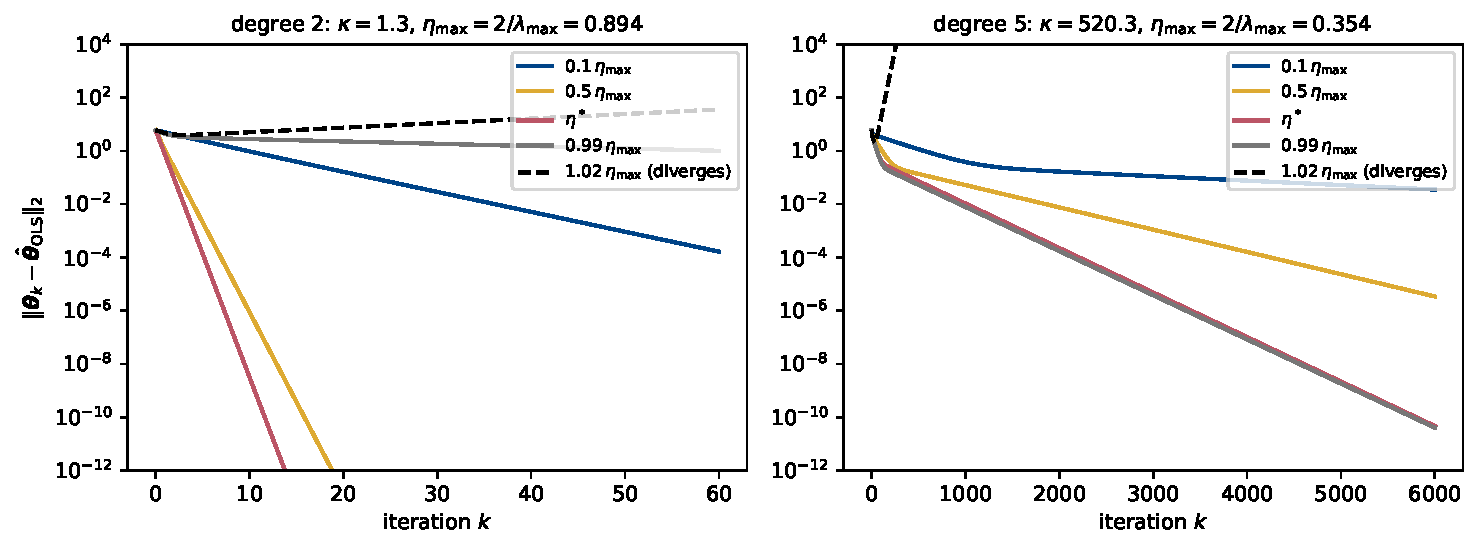
\includegraphics[width=0.98\textwidth]{week37_gd_convergence}
\vspace{1pt}
\footnotesize
$f(x)=2-x+5x^2$ on $[-2,2]$, $n=100$, noise $\sigma=0.5$, standardised
polynomial columns, centred $\bm{y}$ (the week-37 exercises).  \textbf{Left,
degree 2:} $x$ and $x^2$ are nearly uncorrelated on a symmetric interval,
eigenvalues $1.76$ and $2.24$, $\kappa=1.3$: at $\eta^*=0.5$ the closed form
$(-1.077,\,5.855)$ is reached to $10^{-8}$ in 11 iterations; at $\eta=0.01$,
1158.  \textbf{Right, degree 5:} the odd powers $x,x^3,x^5$ are strongly
correlated, eigenvalues from $0.011$ to $5.65$, $\kappa=520$: the best
learning rate needs 4964 iterations, $\eta=0.1$ needs 11\,836, and
$\eta=0.01$ has not converged after $10^5$.  In both panels $1.02\,\eta_{\max}$
diverges -- the boundary of Eq.~(4.20) is sharp.
\end{frame}

\begin{frame}{Scanning the learning rate, and what Ridge does to $\kappa$}
\begin{columns}
\begin{column}{0.54\textwidth}
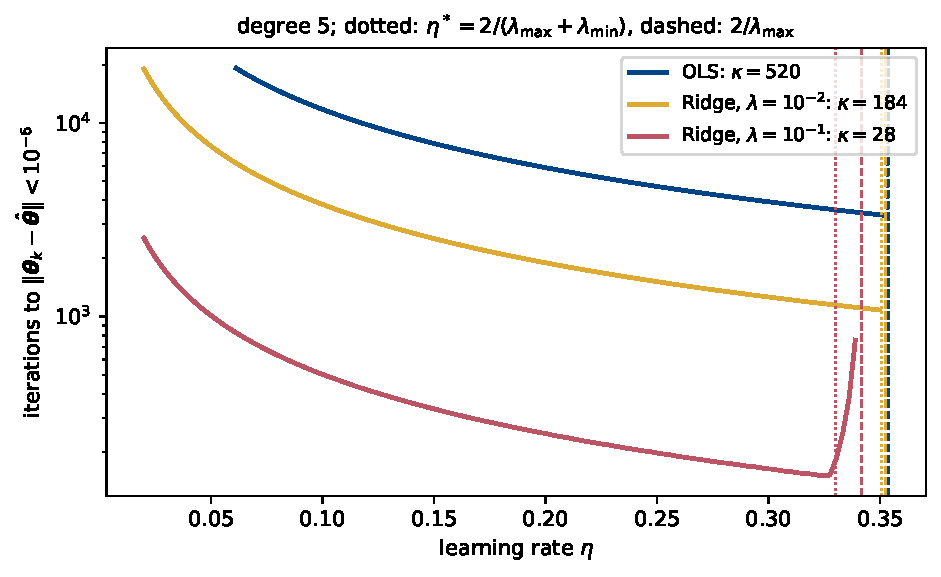
\includegraphics[width=\textwidth]{week37_eta_scan}
\end{column}
\begin{column}{0.45\textwidth}
\footnotesize
Degree-5 exercise data, iterations to $\|\bm{\theta}_k-\hat{\bm{\theta}}\|<10^{-6}$.
\begin{itemize}
  \item OLS: $\kappa=520$; the minimum sits at $\eta^*=0.353$, and $0.354$
        is the edge of the cliff.
  \item Ridge, $\lambda=10^{-2}$: $\lambda_{\min}$ goes from $0.011$ to
        $0.031$, $\kappa=184$, three times fewer iterations at the optimum.
  \item Ridge, $\lambda=10^{-1}$: $\kappa=28$, twenty times fewer.
\end{itemize}
\vspace{3pt}
The penalty lifts the \emph{small} eigenvalues -- the flat directions that
gradient descent crawls along -- and barely touches the large one, so
$\eta_{\max}$ hardly moves while $\eta^*$ does.  Regularisation is good for
the optimiser, not only for the estimator.
\vspace{3pt}
Tuesday, Case 1: you produce both figures with your own code and check the
eigenvalue bound on your own Hessian.
\end{column}
\end{columns}
\end{frame}

\begin{insight}[the $\eta=0.001$ of the old notes]
\question{Last year's notes ran gradient descent for OLS with $\eta=0.001$
and 1000 iterations on the degree-2 exercise data and reported the result as
``converged''.  How far from the closed form was it, roughly?}
\answer{Not converged at all.  With $\lambda_{\min}=1.76$ the slow direction
contracts by $(1-0.001\cdot1.76)^{1000}=e^{-1.76}\approx0.17$ per thousand
iterations: after 1000 steps a sixth of the initial error is still there,
in the \emph{second} digit of $\bm{\theta}$.  A converged run needs
$\|\nabla C\|$ below tolerance, not a fixed iteration count.  And the
converse trap: on this problem $\eta=0.8$ is fine, but move to degree 5 and
$\eta_{\max}=0.354$ -- the safe $\eta$ is a property of the \emph{data}, not
of the algorithm.  Compute $\lambda_{\max}$ of your Hessian; it is one line.}
\end{insight}

%% ====================================================================
%% Part 3 -- momentum (4.6)
%% ====================================================================

\begin{frame}{Momentum: give the iteration a memory (Section 4.6)}
\small
Replace Eq.~(4.10) by
\[
  \boxed{\;\bm{v}_{k+1}=\gamma\bm{v}_k+\eta\nabla C(\bm{\theta}_k),\qquad
  \bm{\theta}_{k+1}=\bm{\theta}_k-\bm{v}_{k+1}\;}\qquad\text{Eq.~(4.23)},
\]
with $\gamma\in[0,1)$ the \textbf{momentum parameter}, typically $0.9$.
Unrolling,
\[
  \bm{v}_{k+1}=\eta\sum_{j=0}^{k}\gamma^{\,k-j}\nabla C(\bm{\theta}_j),
  \qquad\text{Eq.~(4.24)}:
\]
an exponentially weighted sum of \emph{all} gradients seen so far;
$\gamma=0$ is plain gradient descent.
\begin{columns}
\begin{column}{0.49\textwidth}
\footnotesize
\begin{block}{Flat direction, $\eta\lambda_i\ll1$}
Successive gradients point the same way and add up.  A constant gradient
$g$ accumulates to
\[
  v_\infty=\eta g\sum_j\gamma^j=\frac{\eta g}{1-\gamma},\quad\text{Eq.~(4.25)}:
\]
the effective step is multiplied by $1/(1-\gamma)$ -- ten for $\gamma=0.9$.
\end{block}
\end{column}
\begin{column}{0.49\textwidth}
\footnotesize
\begin{block}{Steep direction}
The iterate overshoots, the gradient flips sign every step, successive terms
in Eq.~(4.24) alternate and largely \emph{cancel}: the accumulated step is
\emph{smaller} than the bare gradient.  The oscillation across the valley is
damped.
\end{block}
\end{column}
\end{columns}
\centering\small
Momentum amplifies the consistent and cancels the oscillatory -- the right
treatment for exactly the landscape Eq.~(4.19) diagnosed.
\end{frame}

\begin{frame}{From $\kappa$ to $\sqrt\kappa$ (book Figure 4.3)}
\begin{columns}
\begin{column}{0.48\textwidth}

\includegraphics[width=\textwidth]{momentum_rate}
\end{column}
\begin{column}{0.5\textwidth}
\footnotesize
Along an eigendirection the momentum iteration is a \emph{two-term}
recurrence in $\tilde e$.  With optimally chosen $\eta$ and $\gamma$ its
contraction rate improves from Eq.~(4.21) to
\[
  \frac{\sqrt\kappa-1}{\sqrt\kappa+1},\qquad\text{Eq.~(4.26)}:
\]
iterations scale with $\sqrt\kappa$ instead of $\kappa$.  At $\kappa=10^2$
an order of magnitude saved; at $10^4$, two.  And by Eq.~(4.22) the
least-squares $\kappa$ is the condition number of $\bm{X}$ \emph{squared},
so these values are ordinary.
\vspace{4pt}
$\sqrt\kappa$ is also the rate of conjugate gradients (Section 1.16): both
build the step from the current gradient and the previous direction.
Momentum is conjugate gradients with the optimal coefficients replaced by a
fixed constant that needs no recomputation and no quadratic cost.
\vspace{4pt}
\textbf{Nesterov momentum} evaluates the gradient at the look-ahead point
$\bm{\theta}_k-\gamma\bm{v}_k$: if the velocity is about to overshoot, the
gradient there already points back.  A flag on every framework's optimiser.
\end{column}
\end{columns}
\end{frame}

\begin{frame}{Momentum on the Runge function -- Project 1, parts e) and f)}
\begin{columns}
\begin{column}{0.54\textwidth}
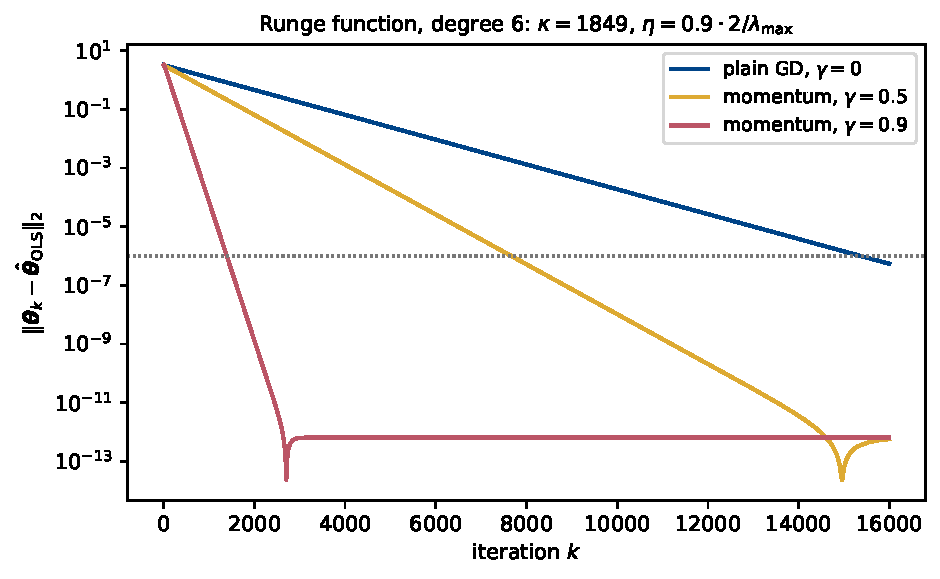
\includegraphics[width=\textwidth]{week37_momentum}
\end{column}
\begin{column}{0.45\textwidth}
\small
$f(x)=1/(1+25x^2)$ on $[-1,1]$, $n=100$, $\sigma=0.1$, degree 6,
standardised columns: $\lambda_{\max}=6.0$, $\lambda_{\min}=0.0032$,
$\kappa=1849$.  Same $\eta=0.9\cdot2/\lambda_{\max}=0.30$ for all three.
\vspace{3pt}
Iterations to $\|\bm{\theta}_k-\hat{\bm{\theta}}_{\mathrm{OLS}}\|<10^{-6}$:
\begin{center}
\begin{tabular}{lr}
\toprule
plain GD, $\gamma=0$ & $15\,374$\\
momentum, $\gamma=0.5$ & $7\,669$\\
momentum, $\gamma=0.9$ & $1\,391$\\
\bottomrule
\end{tabular}
\end{center}
\vspace{2pt}
A factor 11 from a single extra line of code -- in line with Eq.~(4.26),
$\sqrt{1849}=43$ being the ceiling with \emph{tuned} $\eta,\gamma$.  At
degree 10, $\kappa\approx2\times10^6$ and plain gradient descent does not
converge in $10^5$ iterations: this is why part f) of the project exists.
\vspace{3pt}
Tuesday, Case 2: this figure, and its $\eta$-sensitivity, from your own code.
\end{column}
\end{columns}
\end{frame}

\begin{frame}[fragile]{Code: momentum is one line more than gradient descent}
\begin{lstlisting}
def gradient(theta, X, y, lam=0.0):
    """Eqs. (4.13) and (4.17): gradient of (1/n)||X theta - y||^2 + lam theta^T theta."""
    n = len(y)
    return (2.0 / n) * X.T @ (X @ theta - y) + 2.0 * lam * theta

def momentum_descent(X, y, eta, gamma, lam=0.0, num_iters=5000, tol=1e-8):
    """Gradient descent with momentum, Eq. (4.23). gamma = 0 is plain gradient descent."""
    theta, v = np.zeros(X.shape[1]), np.zeros(X.shape[1])
    history = [theta.copy()]
    for t in range(num_iters):
        g = gradient(theta, X, y, lam)
        v = gamma * v + eta * g          # the memory
        theta = theta - v
        history.append(theta.copy())
        if np.linalg.norm(g) < tol:
            break
    return np.array(history), t + 1
\end{lstlisting}
\small
The update rule does not care where \texttt{gradient} comes from -- an
analytical formula, or (next) automatic differentiation.  That separation is
the structure of your Project 1 code: one function for the cost, one for its
gradient, one per optimiser.
\end{frame}

\begin{insight}[why not $\gamma=0.99$?]
\question{If $\gamma=0.9$ multiplies the effective step by 10, why not take
$\gamma=0.99$ for a factor 100, or $0.999$?}
\answer{Two reasons.  First, stability: the two-term recurrence converges
only for $\eta\lambda_{\max}<2(1+\gamma)$ \emph{and} the effective step
$\eta/(1-\gamma)$ along the flat directions must not itself overshoot --
with $\gamma\to1$ the iterate becomes a nearly frictionless ball that rolls
through the minimum and back for ever.  Second, the optimum is
\emph{tied to} $\kappa$: the rate of Eq.~(4.26) is attained at
$\gamma^*=\bigl((\sqrt\kappa-1)/(\sqrt\kappa+1)\bigr)^2$, which is $0.91$
for the Runge problem ($\kappa=1849$) and $0.67$ for $\kappa=100$.  Past
$\gamma^*$ the iteration count \emph{rises} again.  Default $0.9$; tune with
cross-validation if it matters; never $0.999$ blindly.}
\end{insight}

%% ====================================================================
%% Part 4 -- automatic differentiation (4.14)
%% ====================================================================

\begin{frame}{Every method today needs a gradient (Section 4.14)}
For OLS we derived it by hand, Eq.~(4.13).  For a network with a dozen layers
that is possible but error-prone; for a model under active development,
impractical.  \textbf{Automatic differentiation} (AD) solves the problem
completely.
\vspace{4pt}
\begin{block}{The idea}
Every program, however complicated, executes a sequence of elementary
operations -- $+$, $\times$, $\exp$, $\log$, $\sin$ -- each with a known
derivative.  Apply the chain rule to that sequence and you obtain
derivatives of any order, \textbf{accurate to working precision}, at a cost
only a small constant factor above the program itself.  Both halves of that
sentence are theorems.
\end{block}
\vspace{4pt}
Plan for the next fifteen minutes: what AD is \emph{not} (symbolic, numerical);
the evaluation trace; the two modes, forward and reverse, from the chain
rule; the cheap gradient principle; JAX on this morning's problems.
\vspace{4pt}
\centering\small
\emph{Reverse-mode AD is what backpropagation is.}  Chapter 8 will meet it
again under that name.
\end{frame}

\begin{frame}{Three ways to differentiate a program (Section 4.14.1)}
\begin{columns}
\begin{column}{0.47\textwidth}
\textbf{Symbolic.}  Manipulates the \emph{formula}; exact, but needs a single
closed-form expression (no loops, no branches) and suffers expression swell.
\vspace{4pt}
\textbf{Numerical.}  Central difference, Eq.~(4.43),
\[
  D_hf(x)=\frac{f(x+h)-f(x-h)}{2h}=f'(x)+\frac{h^2}{6}f'''(x)+\dots
\]
Truncation error $\propto h^2$ (Eq.~4.44) wants $h$ small; rounding error
$\epsilon_M|f|/h$ wants it large:
\[
  E(h)\approx\frac{h^2}{6}|f'''|+\frac{\epsilon_M|f|}{h},\qquad\text{Eq.~(4.45)}.
\]
\end{column}
\begin{column}{0.51\textwidth}
Minimising, Eq.~(4.46):
\[
  h^*\sim\epsilon_M^{1/3}\approx6\times10^{-6},\qquad
  E(h^*)\sim\epsilon_M^{2/3}\approx4\times10^{-11}.
\]
Two thirds of the digits at best, and only if $h$ is chosen well
(one-sided: $\epsilon_M^{1/2}\approx10^{-8}$).  And the cost: $2p$ function
evaluations per gradient.  For $p=10^7$, a week of computing for one
mediocre gradient.
\vspace{4pt}
\begin{block}{Automatic differentiation has neither defect}
It computes the \emph{value} of the derivative at a point (no swell), by
propagating exact rules through the program (no $h$, no truncation), and in
reverse mode obtains all $p$ components for a small constant number of
function evaluations.
\end{block}
\end{column}
\end{columns}
\end{frame}

\begin{frame}{The evaluation trace and the computational graph (Section 4.14.2)}
\begin{columns}
\begin{column}{0.5\textwidth}
\includegraphics[width=\textwidth]{4-compgraph}
\end{column}
\begin{column}{0.48\textwidth}
\small
AD works not on the formula for $f$ but on the operations a program executes.
For $f(x_1,x_2)=\ln x_1+x_1x_2-\sin x_2$, Eq.~(4.47), the \textbf{evaluation
trace} (Wengert list), Eq.~(4.48):
\[
\begin{aligned}
  v_{-1}&=x_1, & v_0&=x_2,\\
  v_1&=\ln v_{-1}, & v_2&=v_{-1}v_0, & v_3&=\sin v_0,\\
  v_4&=v_1+v_2, & v_5&=v_4-v_3, & y&=v_5.
\end{aligned}
\]
Drawn with an edge $j\to i$ whenever $v_i$ uses $v_j$: the
\textbf{computational graph} (book Figure 4.5).  Loops unroll, branches select
-- \emph{any} program has a trace.  A neural network is a particularly
regular one.
\vspace{3pt}
Each node's \textbf{local derivatives} are known in closed form,
Eq.~(4.49): $\partial v_1/\partial v_{-1}=1/v_{-1}$,
$\partial v_2/\partial v_{-1}=v_0$, $\partial v_2/\partial v_0=v_{-1}$,
$\partial v_3/\partial v_0=\cos v_0$, the rest $\pm1$.
\textbf{All AD does is combine these by the chain rule.  The only question is
in which order.}
\end{column}
\end{columns}
\end{frame}

\begin{frame}{Forward mode: tangents (Section 4.14.3)}
Fix a direction $\dot{\bm{x}}$ in input space and carry with every node its
\textbf{tangent}, the directional derivative
\[
  \dot v_i=\sum_k\frac{\partial v_i}{\partial x_k}\dot x_k,\qquad\text{Eq.~(4.50)},
  \qquad\text{by the chain rule}\qquad
  \dot v_i=\sum_{j\prec i}\frac{\partial\varphi_i}{\partial v_j}\dot v_j,\qquad\text{Eq.~(4.51)}.
\]
Runs in the \emph{same order} as the evaluation, so each tangent is computed
alongside its value.  With $\dot{\bm{x}}=(1,0)$ at $(x_1,x_2)=(2,5)$,
Eq.~(4.52):
\[
\begin{aligned}
  \dot v_{-1}&=1,& \dot v_0&=0,\\
  \dot v_1&=\dot v_{-1}/v_{-1}=0.5,& \dot v_2&=\dot v_{-1}v_0+v_{-1}\dot v_0=5,& \dot v_3&=\cos(v_0)\dot v_0=0,\\
  \dot v_4&=5.5,& \dot v_5&=5.5=\partial f/\partial x_1 .
\end{aligned}
\]
For $\partial f/\partial x_2$: repeat the whole sweep with $\dot{\bm{x}}=(0,1)$.
\vspace{3pt}
\begin{block}{Cost}
One sweep returns $\dot{\bm{y}}=\bm{J}\dot{\bm{x}}$, a \emph{Jacobian--vector
product}, Eq.~(4.55), without forming $\bm{J}$.  The gradient of a scalar
function of $p$ parameters costs $p$ sweeps -- the count of finite
differences, only exact.  Right when the \emph{inputs} are few; wrong for
training.
\end{block}
\end{frame}

\begin{frame}{Dual numbers: forward mode in one line (Section 4.14.3)}
Introduce $\varepsilon$ with $\varepsilon^2=0$, $\varepsilon\ne0$, and the
\textbf{dual numbers} $a+b\varepsilon$:
\[
  (a+b\varepsilon)(c+d\varepsilon)=ac+(ad+bc)\varepsilon,\qquad\text{Eq.~(4.53)},
\]
the product rule as an algebra.  For any $g$ with a Taylor series,
\[
  g(a+b\varepsilon)=g(a)+g'(a)b\varepsilon+\tfrac12g''(a)b^2\varepsilon^2+\dots
  =g(a)+g'(a)\,b\varepsilon,\qquad\text{Eq.~(4.54)}.
\]
The series \emph{terminates} -- by the algebra of $\varepsilon$, not by
neglecting anything.  Evaluate $g$ at $x+1\cdot\varepsilon$ and read off the
coefficient of $\varepsilon$: $g'(x)$, exactly.
\vspace{4pt}
\begin{block}{What this buys}
A dual number carries a value and a derivative together.  Overload the
arithmetic operators of Python so that ordinary code, written with no thought
of derivatives, computes them when handed a dual argument -- next frame,
thirty lines.  This is what \texttt{autograd} does to \texttt{numpy}.
\end{block}
\end{frame}

\begin{frame}[fragile]{Code: a \texttt{Dual} class (book Section 4.14.3)}
\begin{lstlisting}
class Dual:
    """A dual number a + b*eps with eps**2 = 0: a value and its derivative."""
    def __init__(self, val, dot=0.0):
        self.val, self.dot = val, dot
    def _lift(o):
        return o if isinstance(o, Dual) else Dual(o)
    def __add__(self, o):
        o = Dual._lift(o); return Dual(self.val + o.val, self.dot + o.dot)
    __radd__ = __add__
    def __sub__(self, o):
        o = Dual._lift(o); return Dual(self.val - o.val, self.dot - o.dot)
    def __mul__(self, o):               # the product rule, Eq. (4.53)
        o = Dual._lift(o)
        return Dual(self.val * o.val, self.val * o.dot + self.dot * o.val)
    __rmul__ = __mul__

def sin(d): return Dual(math.sin(d.val), math.cos(d.val) * d.dot)   # Eq. (4.54)
def log(d): return Dual(math.log(d.val), d.dot / d.val)

def f(x1, x2):                          # Eq. (4.47), ordinary code
    return log(x1) + x1 * x2 - sin(x2)

print("df/dx1 =", f(Dual(2.0, 1.0), Dual(5.0, 0.0)).dot)   # 1/x1 + x2 = 5.5
print("df/dx2 =", f(Dual(2.0, 0.0), Dual(5.0, 1.0)).dot)   # x1 - cos(x2)
\end{lstlisting}
\end{frame}

\begin{frame}{Reverse mode: adjoints (Section 4.14.4)}
Fix the \emph{output} instead.  For scalar $y$ define the \textbf{adjoint} of
every node, $\bar v_i=\partial y/\partial v_i$, Eq.~(4.56).  Since $y$
depends on $v_j$ only through the nodes that consume it,
\[
  \bar v_j=\sum_{i\succ j}\bar v_i\,\frac{\partial\varphi_i}{\partial v_j},
  \qquad j=\ell-1,\dots,1-n,\qquad\text{Eq.~(4.57)},
\]
started from $\bar v_\ell=1$: the same local derivatives, summed over
\emph{successors}, running \emph{backwards}.  At $(2,5)$, Eq.~(4.58):
\[
\begin{aligned}
  \bar v_5&=1,& \bar v_4&=1,& \bar v_3&=-1,& \bar v_1&=\bar v_2=1,\\
  \bar v_0&=\bar v_3\cos v_0+\bar v_2v_{-1}=2-\cos5=1.716,&
  \bar v_{-1}&=\bar v_2v_0+\bar v_1/v_{-1}=5.5 .
\end{aligned}
\]
\textbf{Both} partial derivatives from \emph{one} sweep.  The two terms in
$\bar v_0$ are the two paths from $v_0$ to $y$ in the graph: the chain rule
sums over paths, and the reverse sweep visits each edge once.
\vspace{3pt}
\begin{block}{The price: the tape}
The local derivatives need the \emph{values} $v_j$ ($\cos v_0$, $v_{-1}$),
in reverse order of production.  The forward evaluation must be recorded;
memory $\propto$ length of the trace.  This is why training a deep network is
memory-bound: every activation of every layer is stored until the backward
pass has consumed it.
\end{block}
\end{frame}

\begin{frame}{The cheap gradient principle (Section 4.14.4)}
For a vector output seeded with a covector $\bar{\bm{y}}$ the reverse sweep
returns $\bar{\bm{x}}=\bm{J}^T\bar{\bm{y}}$, a \emph{vector--Jacobian
product}, Eq.~(4.59) -- the chain rule of Eq.~(1.51) with the products
taken in the cheapest order.
\vspace{4pt}
\begin{block}{Proposition (Baur--Strassen, Linnainmaa)}
Let $f:\mathbb{R}^p\to\mathbb{R}$ be evaluated by a trace of $\ell$
elementary operations with at most two arguments each.  Then reverse-mode AD
computes $f(\bm{x})$ \emph{and the complete gradient} $\nabla f(\bm{x})$ in at
most $c\,\ell$ operations, $c\le4$, \textbf{independent of $p$}.
\end{block}
\emph{Proof sketch.}  The forward evaluation costs $\ell$ and records the tape.
In Eq.~(4.57) each edge $j\to i$ contributes one term -- one multiplication,
one addition, a local derivative that is often free.  At most two incoming
edges per node, so at most $2\ell$ edges.  Nowhere did $p$ enter: it decides
how many adjoints are \emph{read off} at the end, not how many operations
are performed.\hfill$\square$
\vspace{4pt}
In practice $c\approx2$--$3$: \textbf{a gradient costs two or three function
evaluations}, against $p+1$ for finite differences and $p$ sweeps for
forward mode.  For $p=10^7$ this is the difference between a fraction of a
second and a week -- the entire difference between what can and cannot be
trained.  Backpropagation is Eq.~(4.57) specialised to the layered trace of a
network.
\end{frame}

\begin{insight}[which mode for which job?]
\question{(a) Training a network with $p=10^7$ parameters and a scalar loss.
(b) A network with 3 inputs $(x,y,t)$ whose output must satisfy a partial
differential equation, so you need $\partial u/\partial x$,
$\partial u/\partial t$ at many points.  (c) The full $m\times n$ Jacobian of
$\bm{f}:\mathbb{R}^{n}\to\mathbb{R}^{m}$ with $m\approx n$.  Forward or
reverse?}
\answer{Section 4.14.5 writes the Jacobian as the product
$\bm{J}=\bm{J}_L\cdots\bm{J}_1$, Eq.~(4.60); forward multiplies from the
right (cost $\propto n$ sweeps), reverse from the left ($\propto m$ sweeps).
(a) $m=1$, $n=10^7$: reverse, by a factor $10^7$.  (b) $n=3$ inputs, many
outputs: forward -- three sweeps, and \texttt{jvp} gives each directional
derivative directly (Chapter 9 uses exactly this).  (c) Neither wins; the
cheapest bracketing of Eq.~(4.60) is NP-hard in general, use whichever and do
not worry.  Bonus: forward \emph{over} reverse gives Hessian--vector products
$\bm{H}\bm{v}$, Eq.~(4.61), for the price of a few gradients and without ever
forming $\bm{H}$ -- the curvature Newton's method wanted, at a linear price.}
\end{insight}

\begin{frame}[fragile]{JAX: \texttt{grad}, \texttt{jit}, \texttt{vmap} (Section 4.14.7)}
\begin{lstlisting}
import jax
jax.config.update("jax_enable_x64", True)   # double precision throughout -- ALWAYS
import jax.numpy as jnp
from jax import grad, jit, vmap

def f(x):
    return jnp.sin(2 * jnp.pi * x + x**2)

df = grad(f)                       # reverse-mode gradient of a scalar function
print(df(1.0))                     # 4.475424121402227, exact to all digits
print(grad(grad(f))(1.0))          # second derivative, by composing grad

xs = jnp.linspace(0.0, 1.0, 5)
print(vmap(df)(xs))                # the derivative at five points at once
fast_df = jit(df)                  # compiled on first call, then very fast
\end{lstlisting}
\small
JAX combines the differentiation machinery with a compiler (XLA): the same
code is differentiated, compiled, vectorised over a batch and run on a GPU.
Forward and reverse mode are explicit as \texttt{jvp} and \texttt{vjp},
\texttt{jacfwd} and \texttt{jacrev}; \texttt{jax.hessian} is
\texttt{jacfwd(jacrev(f))}.
\begin{block}{Precision}
JAX uses single precision by default.  Without the first line, the gradient
checks that follow agree only to seven digits, and one would wrongly conclude
that AD is inexact.
\end{block}
\end{frame}

\begin{frame}[fragile]{The least-squares gradient without deriving it}
\begin{lstlisting}
Xj, yj = jnp.asarray(X), jnp.asarray(y)             # the data of Section 4.4

def cost(theta, X, y):                              # Eq. (4.12), ordinary code
    return jnp.sum((X @ theta - y)**2) / len(y)

cost_grad = jit(grad(cost, argnums=0))              # d cost / d theta, compiled

theta = jnp.asarray(rng.normal(size=(2, 1)))
g_ad = cost_grad(theta, Xj, yj)
g_hand = (2.0 / n) * X.T @ (X @ np.asarray(theta) - y)   # Eq. (4.13)
print("max |AD - hand| =", np.max(np.abs(np.asarray(g_ad) - g_hand)))   # 5e-15

eta = 0.1
@jit
def gd_step(theta):                                 # Eq. (4.15) with the automatic gradient
    return theta - eta * grad(cost)(theta, Xj, yj)
for k in range(1000):
    theta = gd_step(theta)
\end{lstlisting}
\small
The two gradients agree to $5\times10^{-15}$ -- rounding -- and the iteration
returns the analytical $(4.03012,\,2.80580)$.  \textbf{Do this check once,
as a habit:} comparing an analytical gradient against the automatic one is
the standard way of catching an error in a derivation.  Project 1, part e),
asks for exactly this comparison, for OLS and for Ridge.
\end{frame}

\begin{frame}[fragile]{Ridge, and a derivative nobody asked for}
\begin{lstlisting}
def ridge_cost(theta, X, y, lmbda):                 # Eq. (4.16)
    return jnp.sum((X @ theta - y)**2) / len(y) + lmbda * jnp.sum(theta**2)

lmbda = 0.001
theta = jnp.asarray(rng.normal(size=(2, 1)))
step = jit(lambda th: th - eta * grad(ridge_cost)(th, Xj, yj, lmbda))
for k in range(1000):
    theta = step(theta)

theta_closed = np.linalg.inv(X.T @ X + n * lmbda * np.eye(2)) @ X.T @ y   # the n again
print("gradient descent:", np.asarray(theta).ravel())
print("closed form:     ", theta_closed.ravel())

# the derivative with respect to lambda, argument number 3
dC_dlambda = grad(ridge_cost, argnums=3)(theta, Xj, yj, lmbda)
print(dC_dlambda, "=", jnp.sum(theta**2))           # theta^T theta, by Eq. (4.16)
\end{lstlisting}
\small
Changing the cost changes \emph{one} function; the gradient follows.
And \texttt{grad} differentiates with respect to \emph{any} argument:
$\partial C/\partial\lambda=\bm{\theta}^T\bm{\theta}$ falls out for free --
the kind of quantity one wants when tuning hyperparameters by gradient
methods rather than by grid search.
\end{frame}

\begin{frame}[fragile]{Hessians, one Newton step, and Hessian--vector products}
\begin{lstlisting}
from jax import hessian, jvp

H = hessian(cost)(theta, Xj, yj).reshape(2, 2)      # forward-over-reverse
print(H); print((2.0 / n) * X.T @ X)                # Eq. (4.14), to rounding

theta0 = jnp.asarray(rng.normal(size=(2, 1)))       # one Newton step, Eq. (4.8)
theta_newton = theta0 - jnp.linalg.solve(H, grad(cost)(theta0, Xj, yj))
print("one Newton step:", np.asarray(theta_newton).ravel())   # the exact minimum

def hvp(f, theta, v):                               # Eq. (4.61): H v without H
    return jvp(grad(f), (theta,), (v,))[1]
\end{lstlisting}
\small
Everything this morning promised is now a few lines: the Hessian to rounding,
the single exact Newton step of Eq.~(4.9), and -- for the problems where
$\bm{H}$ cannot be stored -- $\bm{H}\bm{v}$ for the price of a few gradient
evaluations.  Book Section~4.14.8 runs gradient descent, momentum, Adam and
Newton on the non-convex Rosenbrock function with nothing derived by hand:
$27\,206$, $2\,591$, $2\,934$ and $6$ iterations.  Replace the function by a
network with a million parameters and only its definition changes.
\end{frame}

\begin{frame}{Finite differences against automatic differentiation, measured}
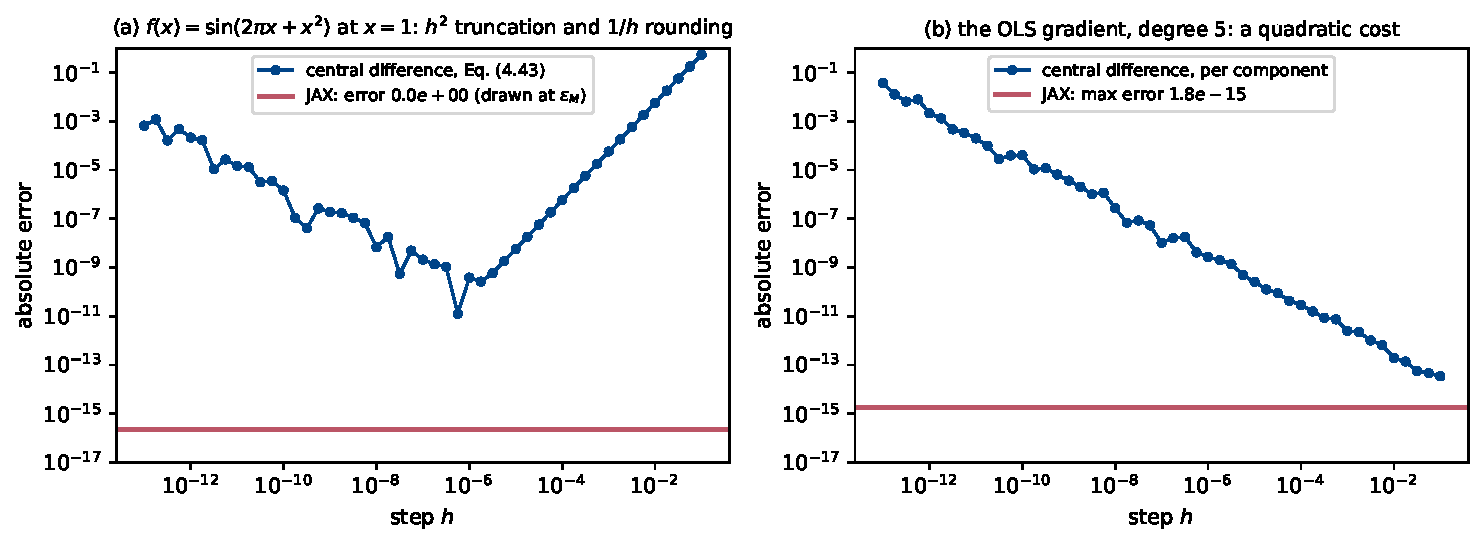
\includegraphics[width=0.98\textwidth]{week37_ad_check}
\vspace{1pt}
\footnotesize
\textbf{(a)} $f(x)=\sin(2\pi x+x^2)$ at $x=1$, book Section 4.14.9: the
error falls as $h^2$ until $h\approx10^{-6}$, then \emph{rises} as $1/h$ --
best $10^{-11}$.  JAX returns $4.475424121402227$, every digit correct.
\textbf{(b)} The degree-5 OLS gradient of this week's exercises, one central
difference per component: the JAX gradient agrees with Eq.~(4.13) to
$1.8\times10^{-15}$ for any $h$, because it involves no $h$.  Whenever you
use a finite-difference check (Eq.~4.63), $h$ must sit at the bottom of the
valley -- and agreement better than $10^{-8}$ should not be expected.
\end{frame}

\begin{insight}[the missing branch]
\question{Panel (b) has no rising $h^2$ branch on the right: the finite
difference of the OLS gradient is \emph{best} at $h=0.1$, with error
$3\times10^{-14}$.  Why -- and does that make finite differences good enough
for Project 1?}
\answer{The OLS cost is a quadratic, so $f'''\equiv0$ and the truncation
term of Eq.~(4.45) vanishes identically: a central difference of a quadratic
is exact for \emph{any} $h$, and only rounding, $\propto1/h$, remains.  Ridge
is quadratic too.  So yes, for parts a)--f) finite differences would pass
the check -- and would still cost $2p$ cost evaluations per gradient against
two or three for reverse mode, and would fail the moment the cost stops being
quadratic (logistic regression next week: panel (a) is the general case).
Use the finite difference as a \emph{check} at $h\approx10^{-5}$; use AD, or
the analytical gradient, for the descent.}
\end{insight}

%% ====================================================================
%% Summary
%% ====================================================================

\begin{frame}{Summary of week 37}
\small
\begin{itemize}
  \item \textbf{Cross-validation} chooses the hyperparameter (Eqs.~3.92--3.96):
        leak-free folds, CV $\pm$ SE, $\lambda_{\min}$ or one-SE, refit,
        test set once.  The bootstrap says which coefficients to believe.
  \item Convex cost $\Rightarrow$ any stationary point is the global minimum
        (Eq.~4.2).  Newton's method, Eq.~(4.8), is the ideal: one exact step
        on OLS, but $\mathcal{O}(p^3)$.
  \item Gradient descent, Eq.~(4.15), replaces $\bm{H}^{-1}$ by a scalar
        $\eta$.  The error decouples along eigendirections, Eq.~(4.19):
        stable iff $\eta<2/\lambda_{\max}$ (Eq.~4.20), iterations
        $\propto\kappa=\lambda_{\max}/\lambda_{\min}$ (Eq.~4.21), and for
        regression $\kappa(\bm{H})=\kappa_2(\bm{X})^2$ (Eq.~4.22): standardise,
        and note that Ridge conditions the problem.
  \item Momentum, Eq.~(4.23), amplifies consistent gradients by
        $1/(1-\gamma)$ and cancels oscillating ones: $\kappa\to\sqrt\kappa$
        (Eq.~4.26).  A factor 11 on the Runge problem from one line.
  \item Automatic differentiation propagates exact derivative rules through
        the evaluation trace: forward mode (tangents, dual numbers), reverse
        mode (adjoints, the tape), and the cheap gradient principle -- a
        gradient for the price of two or three function evaluations,
        independent of $p$.  \texttt{jax.grad} of your cost function
        \emph{is} your gradient; check it once against Eq.~(4.13).
\end{itemize}
\begin{block}{Tomorrow, the deadline, and next week}
Tuesday: Case 1 = your own gradient descent for OLS and Ridge with analytical
gradients, learning rates and stopping; Case 2 = momentum and the JAX
gradient on the Runge function of Project 1.  Exercises due \textbf{Friday
September 11 at midnight}.  Week 38: stochastic gradient descent, AdaGrad,
RMSProp and Adam, applied to Lasso and logistic regression.
\end{block}
\end{frame}

\end{document}
